In order to address the problem raised by Herley, 
we shall define how to distinguish between a secure and an insecure system.
While most of the literature (and this paper so far) have
correlated the problem of in-security to the maliciousness of
agents interacting with the system, we show that security
doesn't seem to have a malicious nature but, rather, insecurity 
raises from the lack of well-defined security requirements for the
design process of a system. We argue that the high number
of security vulnerability reported today are simply the realization
of potential system configurations, which deviate from the nominal
behavior just because the intended behavior of the system is not precisely 
defined in the specification of the design process. 

Given that we apply our theory to \emph{systems engineering} and that
the two foundational processes (exploitation and hacking) are based on the
concept of a system, we shall begin by defining what a system is, in its
abstract form.

\subsection{Abstract Systems}\label{sec:system}
The ISO/IEC/IEEE 15288:2015 (System Life Cycle Processes) provides a definition
of system as ``A combination of interacting elements organized to achieve one
or more stated purposes.''\autocite{ISO201515288}.  Therefore, a system can be
considered as a single agent where its interacting elements are the
constituents of the agent itself. For the sake of simplicity we first define a
system as an agent and then extend the definition to a ``combination of
interacting'' agents.  We use the same process of \autocite{Santaca2016abf} but
over slightly different terms. The differences and commonalities with
\autocite{Santaca2016abf} are described in Appendix~\ref{app:abf}. 

There is no agreement between the research communities (e.g.
Multi-Agent-System, Epistemic Logic) on which are the constituent of an agent
as a system. However, the same ideas revolved around for thousands of years.
Some examples follows.
\begin{itemize}
	\item In \autocite{Georgeoff1995bdi}, the BDI (Belief, Desire, Intent)
		paradigm is explained; where an agent can be defined over those
		three constituents.
	\item In \autocite{Hintikka1962knowledge}, Hintikka describes the
		difference between Knowledge and Belief (as epistemological
		concepts), and the whole Doxastic logic defines in details how
		Beliefs can be formalized.
	\item In \autocite{Hintikka1993Information}, Hintikka describes the concept
		of Information and the difference with Knowledge and Belief.
	\item In \autocite{Empiricus1990Pyrrhonism}, the author states: ``The
		logical criterion also may be used in three senses -- of the
		agent, or the instrument, or the ``according to what''; the
		agent, for instance, may be a man, the instrument either sense
		perception or intelligence, and the ``according to what'' the
		application of the impression ``according to'' which the man
		proceeds to judge by means of one of the aforesaid
		instruments.'' 
	\item In \autocite{Santaca2016abf}, the authors defines an agent as a
		tuple of Assertions, Beliefs, and Facts.
\end{itemize}

If we consider \autocite{Empiricus1990Pyrrhonism}, the author applies a
``logical criterion'' to an agent, for instance a man, for instance a device in
a system (or a system) as in \autocite{Santaca2016abf}.  The instrument identified is sense
perception, because a man is considered as example, but we can abstract the
concept of instrument as any received information, where information is
considered as defined in \autocite{Hintikka1993Information}; which can be
summarized by the following axiom: ``Information is specified by specifying
which alternatives concerning the reality it admits and which alternatives
excludes''. This means, for our argument, that considering a propositional
variable, which admits the two alternatives True/False, its information is
defined as excluding either to be True or False and then, as we'll discuss
later on, Believed to be the opposite. Similarly, when reasoning on a
mereotopological region w.r.t. the RCC (e.g. RCC3 admits two regions to be
equal, disjoint, or overlapping) and information on this region should exclude
some of the alternatives. Finally, in \autocite{Empiricus1990Pyrrhonism}
the author states that the logical criterium can be judged according to something.
For our argument, as in \autocite{Santaca2016abf}, we define this concept
as Knowledge (or Facts); where knowledge is defined, as in \autocite{Steup2020epistemology}, as
a set of proposition known by an agent, such that: (i) knowledge requires belief,
(ii) knowledge require truth, (iii) knowledge must be \emph{properly justified}.

Before detailing what ``properly justified'' means, we discuss the mentioned
relation between agent and belief and we introduce a more formal definition
of knowledge and belief. For our argument, the only objective of
Information is to interact with the behavior of a system or an agent. 
Due to the definition of Information and its relation to the probabilistic
correlation between information and truth/reality, we must consider
information in relation with an agent's beliefs. Similarly, we consider
beliefs to define the behavior of an agent or a system. On the other hand,
Knowledge drives the nominal behavior of an agent or a system. This view
is not considered in most (if not all) the approaches to protocol verification
and the Dolev-Yao theory is usually applied to a representation/abstraction
of a protocol that only considers knowledge and transfer of knowledge (i.e.
if an agent sends a message, the recipient knows that message). However,
the security of a system is tightly related to the difference between
the nominal behavior and the implemented one.

\begin{definition}{\bf System --}\label{def:system}
	A system (or a sub-system) is an agent (see Definition~\ref{def:agent})
	such that
	$s=\langle\rcc(\knowledgeRegion,\beliefRegion),\rcc(\knowledgeRegion,\informationRegion),\rcc(\beliefRegion,\informationRegion)\rangle$,
	where $\knowledgeRegion,\beliefRegion,\informationRegion$ are Regions of Knowledge, Beliefs, and Information respectively.
\end{definition}
A system is then defined as a superposition of multiple states where knowledge,
beliefs, and information are related between each other (in a mereotopological
space) through the RCC. A \emph{system instance} is a specific definition of
the $\rcc$ relations between the three regions. Therefore, a set of 
system instances defines a set of choices for those $\rcc$ relations.

% \item  ``normally concern the state or the history of the entire universe but only
% of some small part of
% it''.  
% \item  ``Information and probability are inversely related'', i.e. ``
% the more alternatives a proposition admits of, the more probable and the less
% informative it is, and vice versa''

\begin{figure}[t]
	\centering
	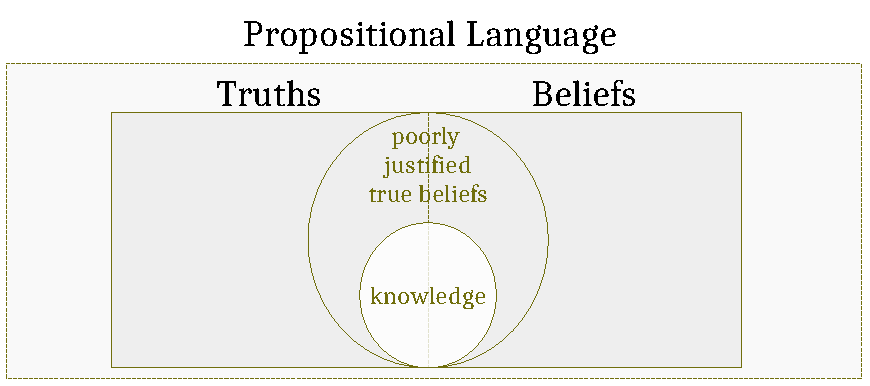
\includegraphics[width=.8\textwidth]{knowledge-belief.pdf}
	\caption{Informal representation of Knowledge and Belief}
	\label{fig:knowledge-belief}
\end{figure}

The difference between Knowledge and Belief is depicted in
Figure~\ref{fig:knowledge-belief} (see \autocite{wiki-knowledgebelief}).  However,
according to\autocite{Gettier2012knowledge},
Knowledge\footnote{``\emph{Theaetetus}: [\ldots] He said that knowledge was
true opinion accompanied by reason, but that unreasoning true opinion was
outside of the sphere of knowledge; and matters of which there is not a
rational explanation are unknowable -- yes, that is what he called them -- and
those of which there is are knowable. [\ldots] \emph{Socrates}: [\ldots] the
primary elements of which we and all else are composed admit of no rational
explanation; for each alone by itself can only be named, and no qualification
can be added, neither that it is nor that it is not, for that would at once be
adding to it existence or non-existence, whereas we must add nothing to it, if
we are to speak of that itself alone.  [\ldots]'' Plato -- Theaetetus 201
\autocite{Plato1914Plato}} as an epistemological concept is difficult to formally define. 
Similarly for the concept of information, Hintikka in \autocite{Hintikka1993Information}
states that ``A purely logical definition of information is impossible''.
In this work, however, we are not interested in how knowledge, information, or
belief can be precisely formalized from an epistemic standpoint.  We assume
that a semantic of a correct definition of epistemic knowledge exists, for
example the one given in\autocite{Hintikka1962knowledge} by Hintikka, and we
then define knowledge in terms of the Kripke structure defined in
Definition~\ref{def:modallogic}; similarly for Belief.

\begin{definition}{\bf Knowledge --}\label{def:knowledge}
Given an abstract collection of Agents $Ag$, and the modal operator
	$\knows{a}{}$ (where $a\in Ag$), Knowledge is defined as a collection
	of predicates known by an agent $\knowledge{a}=\bigcup_\Phi \knows{a}{\varphi}$ 
	(where $\Phi$ is the collection of all the propositions known by $a$).
	Given a proposition $P$, we extend the semantics of the Causality structure with:
	\begin{enumerate}[noitemsep]
		\item[$(\interpretation16)$] $\world\models\knows{a}{P}$ iff
			$\world'\models P$ for all $\world'$ such that
			$\world\modalrelation\world'$.
	\end{enumerate}
\end{definition}

\begin{definition}{\bf Belief --}\label{def:belief}
	Given an abstract collection of Agents $Ag$, and the modal operator
	$\believe{a}{}$ (where $a\in Ag$), Belief is defined as a collection
	of predicates believed by an agent $\belief{a}=\bigcup_\Phi \believe{a}{\varphi}$
	(where $\Phi$ is the collection of all the propositions believed by $a$).
	Given a proposition $P$, we extend the semantics of the Causality structure with:
	\begin{enumerate}[noitemsep]
		\item[$(\interpretation17)$] $\world\models\believe{a}{P}$ iff
			$\world\models\neg\knows{a}{\neg P}$ (i.e. the agent $a$ considers $P$ possible) 
			and $\world'\models P$ for all
			$\world'$ such that $\world\modalrelation\world'$.
	\end{enumerate}
\end{definition}

\begin{definition}{\bf Information --}\label{def:information}
	Given an abstract collection of Agents $Ag$, and the modal operator
	$\informs{a}{}$ (where $a\in Ag$), Information is defined as a collection
	of beliefs asserted by an agents $a$.
	%and transferred from $a$ to $b$ ($a\rightarrow b$).
	$\information{a}=\bigcup_\Phi \informs{a}{}{\varphi}$
	(where $\Phi$ is the collection of all the propositions believed and asserted by $a$).
	Given a proposition $P$, we extend the semantics of the Causality structure with:
	\begin{enumerate}[noitemsep]
		\item[$(\interpretation18)$] $\world\models\informs{a}{P}$ iff
			$\world\models\neg\knows{a}{\neg P}$ (i.e. the agent $a$ considers $P$ possible) 
			and $\world'\models P$ for all
			$\world'$ such that $\world\modalrelation\world'$.
	\end{enumerate}
\end{definition}

When dealing with a specification of a system (i.e. the design if the system
for a specific operation (as a generic operating/operational system),
considering information may be an over-complication since we are usually not
interested in the information in abstract but to the transfer of that
information, which we call Assertions. Therefore, we consider information only
if there is a sender and a recipient.  Similarly, the portion of Beliefs we
consider is the one that builds the behavior of an agent and we consider a set
of axiomatic Facts instead of Knowledge.

\begin{definition}{\bf Assertion}\label{def:assertion}
\end{definition}
\begin{definition}{\bf Behavior}\label{def:behavior}
\end{definition}
\begin{definition}{\bf Fact}\label{def:fact}
\end{definition}

\begin{definition}{\bf Operational System --}\label{def:system}
	An operational system (or a sub-system) is an agent (see Definition~\ref{def:agent})
	such that
	$s=\langle\rcc(\factRegion,\behaviorRegion),\rcc(\factRegion,\assertionRegion),\rcc(\behaviorRegion,\assertionRegion)\rangle$,
	where $\factRegion,\behaviorRegion,\assertionRegion$, are regions of facts, behavior, and assertions respectively.
\end{definition}

As already presented in \autocite{Santaca2016abf} it follows that, defining
a system (or an operational system) with 3 regions, there exist
an upper-bound to the number of possible configuration of a system, defined by
the possible relations between the different regions.
For completeness we report in  stated in the next paragraph
the calculation done in \autocite{Santaca2016abf}.

\Paragraph{Number of different configurations of a system}
\fix{mr}{
The general formula to calculate the number of different types of agents is
$r^{\binom{n}{k}}$, where $r$ is the number of relations with arity $k$,
between $n$ different sets, where $r^e$ is the number of permutation of $r$
relations over $e$ elements with repetitions, with $e$ being the number of
$k$-ary combinations of $n$ sets, $\binom{n}{k}$.
%and the proof is given in the appendix (Section~\ref{app:proof}).
In our case, $\binom{n}{k}=3$ since we consider $3$ sets
($\assertionRegion,\beliefRegion,\factRegion$), and all the relations
considered in the RCC are binary.  Hence, using RCC5 (with five different
spatial relations) over three sets, we can theoretically define up to 125
different type of agents. However, only 54 of the 125 (as showed in
\cite{improvingRCC} and derived by the composition table of RCC5 in
Table~\ref{tab:5com}) combinations are topologically correct with respect to
the definition of the relations of RCC5. Generalizing to all the RCCs, in
Table~\ref{tab:relations} we calculate the number of different agents with
respect to all the variations of RCC (i.e., with 3, 5 or 8 spatial relations).

\begin{itemize}
\item \emph{RCC3} --- theoretical: $3^3=27$,  correct: 15 
\item \emph{RCC5} --- theoretical: $5^3=125$, correct: 54
\item \emph{RCC8} --- theoretical: $8^3=512$, correct: 193
\end{itemize}

Hence, even if considering a different number of sets than the three
$\assertionRegion$, $\behaviorRegion$ and $\factRegion$ exponentially affects
the number of theoretical agents, the application of RCC downscales that number
of a factor that ranges from 1.8 to 2.5. In addition, using RCC5 we consider
3.6 times more (different) types of agents than RCC3, but using RCC8 would
allow us to consider 3.5 times more different agents.}

